\documentclass{beamer}
\usepackage{beamerthemesplit}
\usepackage{wrapfig}
\usetheme{SPbGU}
\usepackage{pdfpages}
\usepackage{amsmath}
\usepackage{cmap} 
\usepackage[T2A]{fontenc} 
\usepackage[utf8]{inputenc}
\usepackage[english,russian]{babel}
\usepackage{indentfirst}
\usepackage{tikz}
\usepackage{multirow}
\usepackage[noend]{algpseudocode}
\usepackage{algorithm}
\usepackage{algorithmicx}
\usetikzlibrary{shapes,arrows}
%usepackage{fancyvrb}
%\usepackage{minted}
%\usepackage{verbments}


\newtheorem{rutheorem}{Теорема}
\newtheorem{ruproof}{Доказательство}
\newtheorem{rudefinition}{Определение}
\newtheorem{rulemma}{Лемма}
\beamertemplatenavigationsymbolsempty

\title[CFPQ]{Структурное представление результата поиска путей с контекстно-свободными ограничениями}
%\subtitle[YaccConstructor]{Parsing techniques for graph analysis}
% То, что в квадратных скобках, отображается в левом нижнем углу. 
\institute[СПбУ]{
JetBrains Research, лаборатория языковых инструментов \\
Санкт-Петербургский университет
}

% То, что в квадратных скобках, отображается в левом нижнем углу.
\author[Семён Григорьев]{Семён Григорьев}

\date{21.10.2017}

\definecolor{orange}{RGB}{179,36,31}

\begin{document}
{
\begin{frame}[fragile]
  \begin{tabular}{p{2.5cm} p{5.5cm} p{2cm}}
   \begin{center}
      
\includegraphics[height=1.5cm]{pictures/JBLogo3.pdf}
    \end{center}
    &
    \begin{center}
      
\includegraphics[height=1cm]{pictures/logo-2017-transp.png}
    \end{center} 
    &
    \begin{center}
      
\includegraphics[height=1.5cm]{pictures/SPbGU_Logo.png}
    \end{center}
  \end{tabular}
  \titlepage
\end{frame}
}


\begin{frame}[fragile]
  \transwipe[direction=90]
  \frametitle{Поиск путей в графах}
  \begin{itemize}
  \item Графовые базы данных
  \item Статический анализ программ
      \begin{itemize}
        \item Анализ алиасов
        \item Статический анализ динамически формируемого кода
        \item ...
      \end{itemize}
   \item ...
  \end{itemize}
\end{frame}

\begin{frame}[fragile]
  \transwipe[direction=90]
  \frametitle{Поиск путей с контекстно-свободными ограничениями}
  \begin{itemize}
  \item $\mathbb{G} = (\Sigma, N, P)$ --- контекстно-свободная грамматика, $L\subseteq \Sigma$
  \item $p=(v_0,l_0,v_1),\cdots,(v_{n-1},l_{n-1},v_n)$ --- путь в графе $G$
  \item $w(p) = w((v_0,l_0,v_1),\cdots,(v_{n-1},l_{n-1},v_n)) = l_0 l_1 \cdots l_{n-1}$
  \item $G = (V,E,L)$ --- ориентированный граф, $E \subseteq V\times L \times V$
  \item $R =\{ p | \exists N_i \in N (w(p) \in L(\mathbb{G},N_i))\}$
  \begin{itemize}
    \item Стартовый нетерминал можно зафиксировать заранее
    \item \textbf{Проблема:} множество $R$ может быть бесконечным
  \end{itemize}
  \end{itemize}
\end{frame}

\begin{frame}[fragile]
  \transwipe[direction=90]
  \frametitle{Существующие решения}
\end{frame}

\begin{frame}[fragile]
  \transwipe[direction=90]
  \frametitle{Алгоритм выполнения КС запросов к графам}

\begin{itemize} 
\item Основан на обобщённом LL (Generalized GLL, GLL)
\begin{itemize} 
  \item Scott E., Johnstone A. GLL parsing
\end{itemize}
\item Поддерживает произвольные контекстно-свободные граммтики (неоднозначные, леворекурсивные)
\item Не требует преобразования грамматики в нормальную форму Хомсого
\item Строит сжатое представление леса разбора (Sharep Packed Parse Forest, SPPF)
\end{itemize}
\end{frame}


\begin{frame}[fragile]
  \transwipe[direction=90]
  \frametitle{Пример}
\begin{figure}[ht]
    \centering
        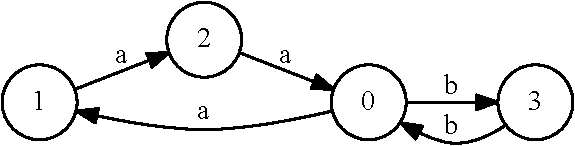
\includegraphics[width=0.45\textwidth]{pictures/input.pdf}
        \caption{Входной граф}
\end{figure}
\begin{figure}[ht]
\centering
   \[
\begin{array}{rl} 
   0:& S \rightarrow a \ S \ b \\
   1:& S \rightarrow Middle \\
   2:& Middle \rightarrow a \ b
\end{array}
\]
   \caption{Запрос: грамматика $G$ для языка $L=\{a^n b^n; n \geq 1\}$ с явным выделением середины пути}
   \label{grammarG}        
    \end{figure}

\end{frame}

\begin{frame}[fragile]
  \transwipe[direction=90]
  \frametitle{Пример: SPPF}
\begin{figure}[ht]
    \centering
        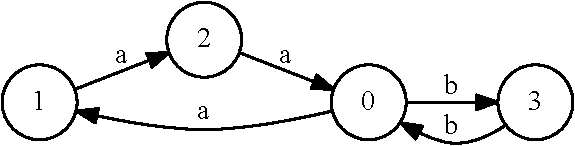
\includegraphics[width=0.45\textwidth]{pictures/input.pdf}
        \caption{Входной граф}
\end{figure}

\begin{tabular}{  c  c  c  }
      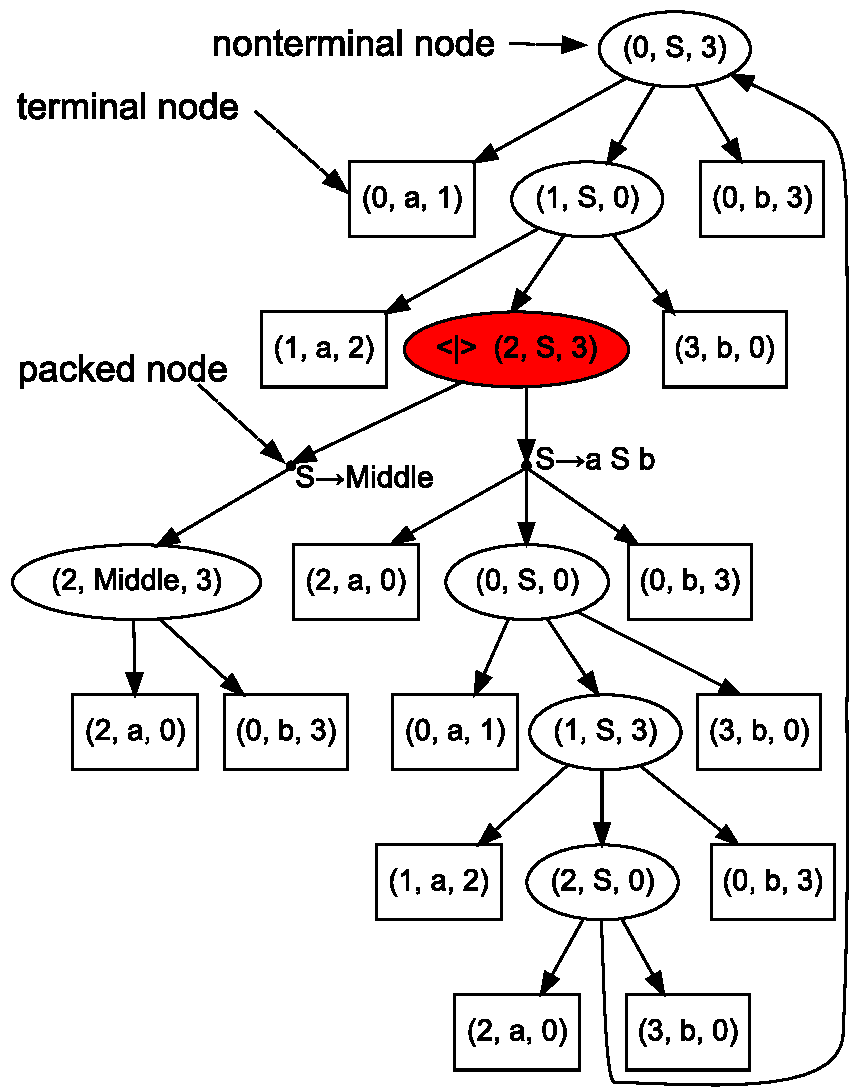
\includegraphics[height=4.5cm]{pictures/AnBn.pdf}
    &
      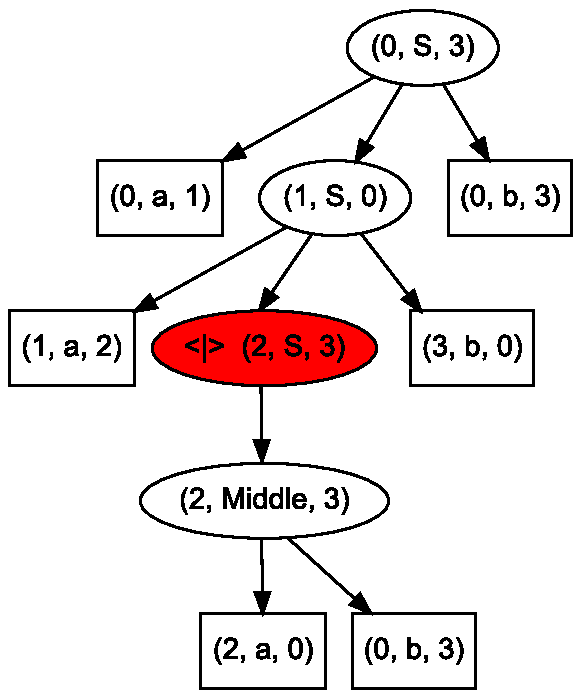
\includegraphics[height=4.5cm]{pictures/AnBn_2.pdf}
    &
      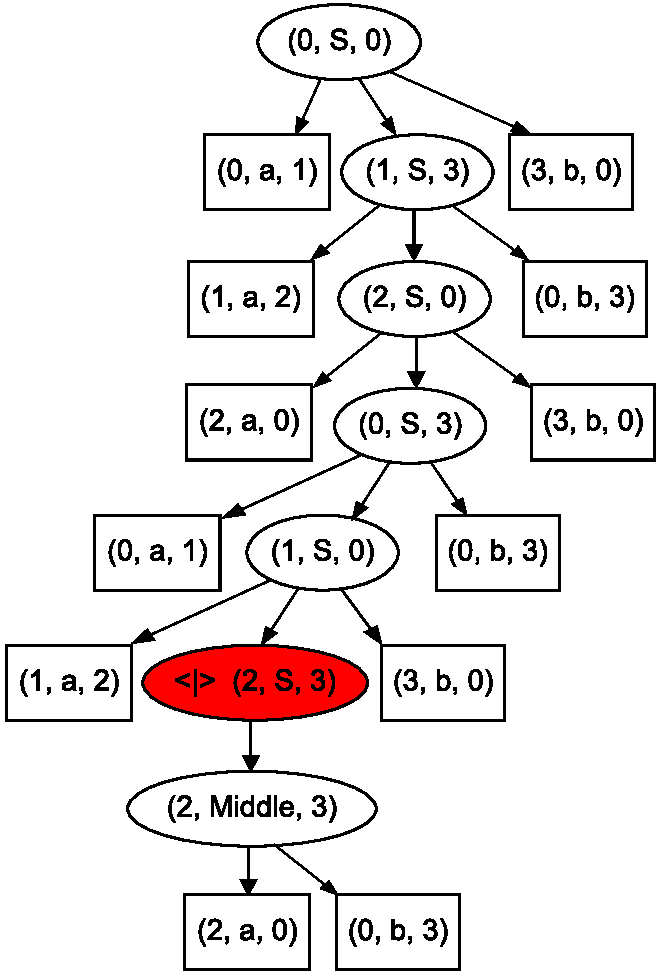
\includegraphics[height=4.5cm]{pictures/AnBn_1.pdf}

\\
Результат
& Структура пути1 
& Структура пути2
  \end{tabular}
%\end{center}                
\end{frame}

\begin{frame}[fragile]
  \transwipe[direction=90]
  \frametitle{Пример: извлечение путей}
\begin{center}
\begin{tabular}{  c  c  }
    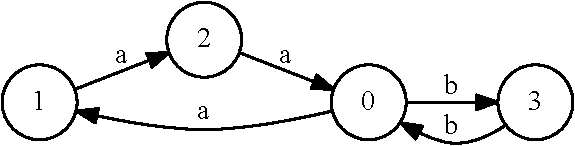
\includegraphics[width=0.4\textwidth]{pictures/input.pdf}
    &
$
 
\begin{array}{rl} 
   0:& S \rightarrow a \ S \ b \\
   1:& S \rightarrow Middle \\
   2:& Middle \rightarrow a \ b
\end{array}

$
\end{tabular}

\begin{figure}[ht]
    \centering
        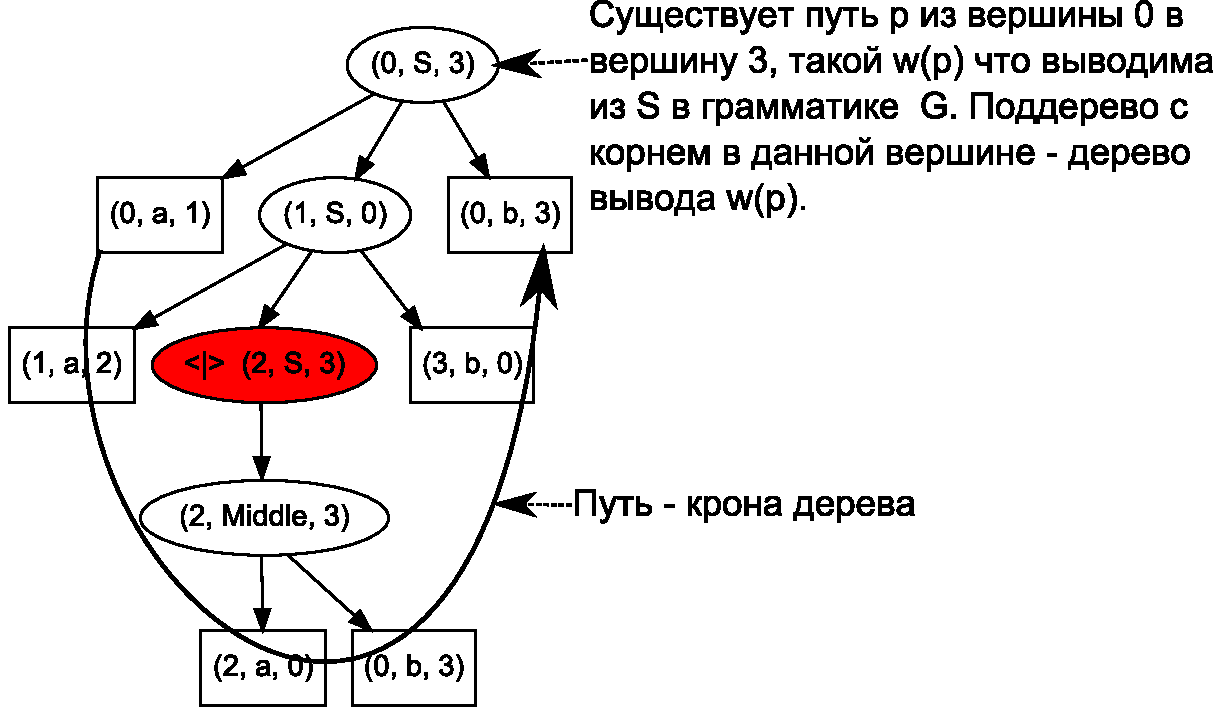
\includegraphics[width=0.68\textwidth]{pictures/AnBn_2_m.pdf}      
\end{figure}
Путь: $(0,a,1);(1,a,2);(2,a,0);(0,b,3);(3,b,0);(0,b,3)$
\end{center}                
\end{frame}


\begin{frame}[fragile]
  \transwipe[direction=90]
  \frametitle{Пример: почему это работает}
Замкнутость КС языков относительно пересечения с регуляными
\begin{center}
\begin{tabular}{  c  c  }
    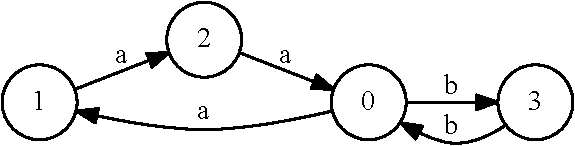
\includegraphics[width=0.35\textwidth]{pictures/input.pdf}
    &
$
 
\begin{array}{rl} 
   0:& S \rightarrow a \ S \ b \\
   1:& S \rightarrow Middle \\
   2:& Middle \rightarrow a \ b
\end{array}

$
\\
Регулярный язык
&
Контекстно-своодный язык

\end{tabular}

\vspace{0.8em}
\pause

\begin{tabular}{  c  c  }
    \raisebox{-0.5\totalheight}{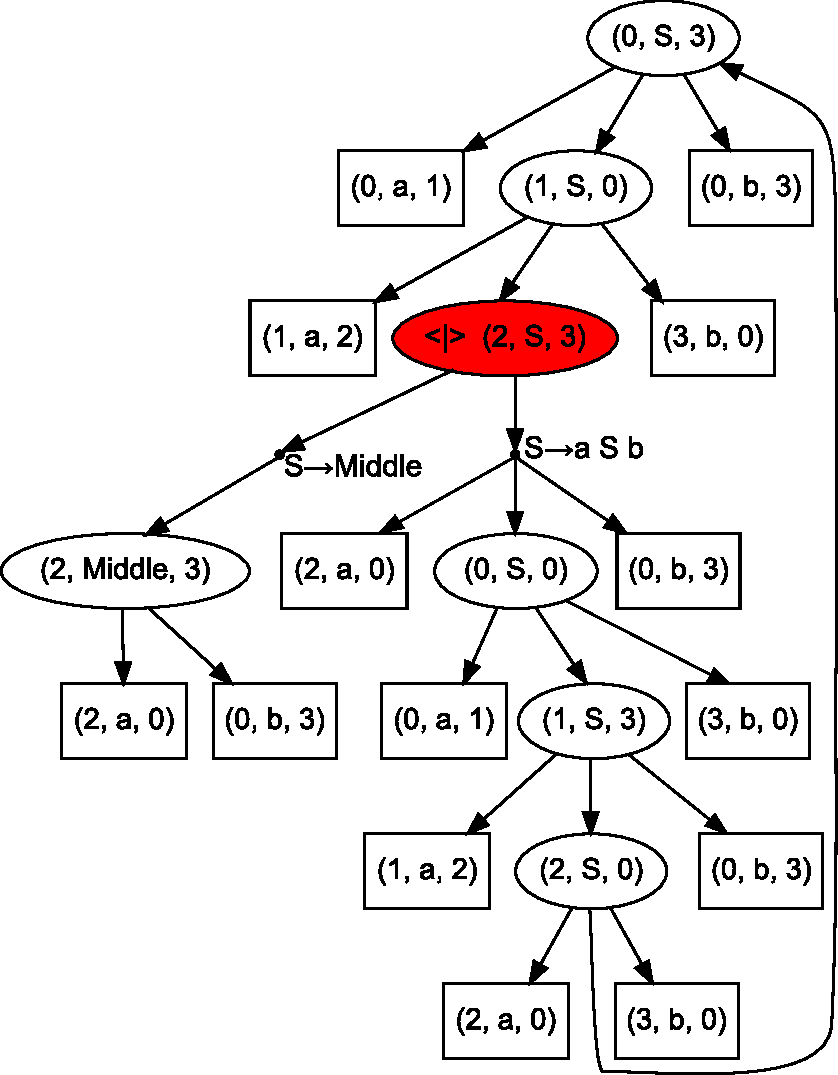
\includegraphics[width=0.32\textwidth]{pictures/AnBn_m.pdf}}
    &

$
\begin{array}{rl} 
   (0,S,3) & \rightarrow (0,a,1) \ (1,S,0) \ (0,b,3) \\
   (1,S,0) & \rightarrow (1,a,2) \ (2,S,3) \ (3,b,0) \\
   (2,S,3) & \rightarrow (2,a,0) \ (0,S,0) \ (0,b,3) \\
   (2,S,3) & \rightarrow (2,Middle,3)                \\
   (0,S,0) & \rightarrow (0,a,1) \ (1,S,3) \ (3,b,0) \\
   (1,S,3) & \rightarrow (1,a,2) \ (2,S,0) \ (0,b,3) \\
   (2,S,0) & \rightarrow (2,a,0) \ (0,S,3) \ (3,b,0) \\
   (0,Middle,3) & \rightarrow (2,a,0) \ (0,b,3)  \\
\end{array}
$

\end{tabular}
\end{center}                
\end{frame}



\begin{frame}
  \transwipe[direction=90]
  \frametitle{Характеристики алгоритма}

Пусть на входе граф $M=(V,E,L)$, тогда
\begin{itemize} 
\item Пространственная сложность предложенного алгоритма равна $O(|V|^3 + |E|)$
\item Временная сложность предложенного алгоритма равна $O\left(|V|^3*\max\limits_{v \in V}\left(deg^+\left(v\right)\right)\right)$
\item Результирующий SPPF имеет размер $O(|V'|^3 + |E'|)$ где $M'=(V',E',L')$ --- это подграф $M$ содержащий только искомые пути
\end{itemize}

\end{frame}

\begin{frame}[fragile]
\transwipe[direction=90]
\frametitle{Экспериментальное исследование: запросы}
%\centering
\begin{figure}[ht]
%   \begin{center}
   \centering
%   \begin{subfigure}[b]{0.4\textwidth}

   \[
\begin{array}{rl}
   0: & S \rightarrow \text{\textit{subClassOf}}^{-1} \ S \ \text{\textit{subClassOf}} \\ 
   1: & S \rightarrow \text{\textit{type}}^{-1} \ S \ \text{\textit{type}} \\ 
   2: & S \rightarrow \text{\textit{subClassOf}}^{-1} \ \text{\textit{subClassOf}} \\ 
   3: & S \rightarrow \text{\textit{type}}^{-1} \ \text{\textit{type}} \\ 
\end{array}
\]
   \caption{Грамматика для запроса Query 1}
   \label{grammarQ1}
   \end{figure}
\begin{figure}[h]%{0.4\textwidth}
   \centering

   \[
\begin{array}{rl}
   0: & S \rightarrow B \ \text{\textit{subClassOf}} \\ 
   1: & S \rightarrow \text{\textit{subClassOf}} \\ 
   2: & B \rightarrow \text{\textit{subClassOf}}^{-1} \ B \ \text{\textit{subClassOf}} \\
   3: & B \rightarrow \text{\textit{subClassOf}}^{-1} \ \text{\textit{subClassOf}} \\ 
\end{array}
\]
   \caption{Грамматика для запроса Query 2}
   \label{grammarQ2}        
   \end{figure}

\end{frame}


\begin{frame}[fragile]
\transwipe[direction=90]
\frametitle{Экспериментальное исследование: результаты}
\centering
\begin{tabular}{ | c | c | c | c | c | c | c |}
\hline
Ontology & \#edg & \multicolumn{3}{|c|}{Query 1} & \multicolumn{2}{|c|}{Query 2} \\
\cline{3-7}
& & \shortstack{time \\ CYK (ms)} & \shortstack{time \\ (ms)} & \#result & \shortstack{time \\ (ms)} & \#result \\
\hline 
\hline
skos        & 252  & 1044  & 10 & 810 & 1 & 1 \\
generations & 273  & 6091  & 19 & 2164 & 1 & 0 \\
travel      & 277  & 13971 & 24 & 2499 & 1 & 63 \\
univ-bench  & 293  & 20981 & 25 & 2540 & 11 & 81 \\
foaf        & 631  & --    & 39 & 4118 & 2 & 10 \\
people-pets & 640  & 82081 & 89 & 9472 & 3 & 37 \\
funding     & 1086 & --    & 212 & 17634 & 23 & 1158 \\
atom-primitive & 425 & 515285 & 255 & 15454 & 66 & 122 \\
\shortstack{biomedical- \\ measure-primitive} & 459 & 420604 & 261 & 15156 & 45 & 2871 \\
pizza       & 1980 & 3233587 & 697 & 56195 & 29 & 1262 \\
wine        & 1839 & 4075319 & 819 & 66572 & 8 & 133 \\
\hline
\end{tabular}

\end{frame}
            
\begin{frame}
\transwipe[direction=90]
\frametitle{Контакты}
\begin{itemize}
  \item Почта: \url{semen.grigorev@jetbrains.com}
  \item GitHub-сообщество YaccConstructor: \url{https://github.com/YaccConstructor}
\end{itemize}
\end{frame}
\end{document}
